\section{Determinantal Point Processes}

A DPP is a distribution over subsets of a fixed ground set.  The essential characteristic of a DPP is that the occurrences of the element of the ground set are negatively correlated, i.e. the inclusion of one item
makes the inclusion of other items less likely. The strengths of these negative correlations are derived from a kernel matrix that defines a global measure of similarity between pairs of items, so that more similar items are less likely to co-occur. As a result, DPPs assign higher probability to sets of items that are diverse.


For the history, Determinantal point processes were first identify as a class by Macchi, who called them "fermion process" because they give the distributions of fermion systems at thermal equilibrium. The Pauli exclusion principle states that no two fermions can occupy the same quantum state; as a consequence fermions exhibit what is known as the
"anti-bunching" effect. This repulsion is described precisely by a DPP.

\subsection{Definition}
Determinantal Point Processes are before all point processes, which can be described as processes for selecting a collection of mathematical points randomly located on a mathematical space. Formally, a point process $\PP$ on a ground set $\mathcal{X}$ is a probability measure over "point patterns" or "point configurations" of $\mathcal{X}$, which are subsets of $\mathcal{X}$. For instance, $\mathcal{X}$ could be a continuous region of the euclidean plane in which a scientist injects some quantum particles trapped into a potential well. Then $\PP\left(\left\{x_1, x_2, x_3\right\}\right)$ characterizes the likelihood of seeing these particles at places $x_1, x_2$, and $x_3$. Depending on the type of the particles, the measurements might tend to cluster together, or they might occur independently, or they might tend to spread out into space. $\PP$ captures these correlations.

In the following, we focus on discrete, finite point processes, where we assume without loss of generality that $\mathcal{X}=\begin{Bmatrix}
    x_{i} \mid i\in \intint{1}{n}
    \end{Bmatrix}$, in this setting we sometimes refer to elements of $\mathcal{X}$ as items. The discrete setting is computationally simpler and often more appropriate for real-world data.

In the discrete case, a point process is simply a probability measure on $2^{\mathcal X}$ i.e. the power set of $\PP$ i.e. the set of all subsets of $\mathcal{X}$. A sample from $\PP$ might be the empty set, the entirety of $\mathcal{X}$, or anything in between. $\PP$ is called a determinantal point process if, when $\mathcal{S}$ is a random subset drawn according to $\PP$, we have, for every $A \subseteq \mathcal{X}$,
\begin{equation}
	\PP(A \subseteq \mathcal{S})=\operatorname{det}\left(K_A\right)
    \label{def_dpp}
\end{equation}
for some real, symmetric $N \times N$ matrix $K$ indexed by the elements of $\mathcal{X}$. Here, $K_A \equiv$ $\left[K_{i j}\right]_{i, j \in A}$ denotes the restriction of $K$ to the entries indexed by elements of $A$, and we adopt $\operatorname{det}\left(K_\emptyset\right)=1$. Note that normalization is unnecessary here, since we are defining marginal probabilities that need not sum to $1$ .

Since $\PP$ is a probability measure, all principal minors $\operatorname{det}\left(K_A\right)$ of $K$ must be nonnegative, and thus $K$ itself must be positive. It is possible to show in the same way that the eigenvalues of $K$ are bounded above by one. These requirements turn out to be sufficient. By the Macchi-Soshnikov theorem (\cite{macchi1975dpp}),any $K$ such that $0 \preceq K \preceq I$, defines a DPP.

We refer to $K$ as the marginal kernel since it contains all the information needed to compute the probability of any subset $A$ being included in $\mathcal{S}$. A few simple observations follow from \ref{def_dpp}. If $A=\{i\}$ is a singleton, then we have
\begin{equation*}
	\PP(i \in \mathcal{S})=K_{i i}
\end{equation*}
That is, the diagonal of $K$ gives the marginal probabilities of inclusion for individual elements of $\mathcal{X}$. Diagonal entries close to 1 correspond to elements of $\mathcal{X}$ that are almost always selected by the DPP. Furthermore, if $A=\{i, j\}$ is a two-element set, then
\begin{equation}
	\begin{aligned}
        \PP(i, j \in \boldsymbol{X}) &=\left|\begin{array}{ll}
	K_{i i} & K_{i j} \\
	K_{j i} & K_{j j}
	\end{array}\right| \\
	&=K_{i i} K_{j j}-K_{i j} K_{j i} \\
	&=\PP(i \in \boldsymbol{X}) \PP(j \in \boldsymbol{X})-K_{i j}^2
	\end{aligned}
    \label{eqn_paircorrel}
\end{equation}
Thus, the off-diagonal elements determine the negative correlations between pairs of elements: large values of $K_{i j}$ imply that $i$ and $j$ tend not to co-occur.

Equation \ref{eqn_paircorrel} demonstrates why DPPs are "diversifying". If we think of the entries of the marginal kernel as measurements of similarity between pairs of elements in $\mathcal{X}$, then highly similar elements are unlikely to appear together. If $K_{i j}=\sqrt{K_{i i} K_{j j}}$, then $i$ and $j$ are "perfectly similar" and do not appear together almost surely. Conversely, when $K$ is diagonal there are no correlations and the elements appear independently. Note that DPPs cannot represent distributions where elements are more likely to co-occur than if they were independent: correlations are always negative.
\begin{figure}[!h]
    \centering
    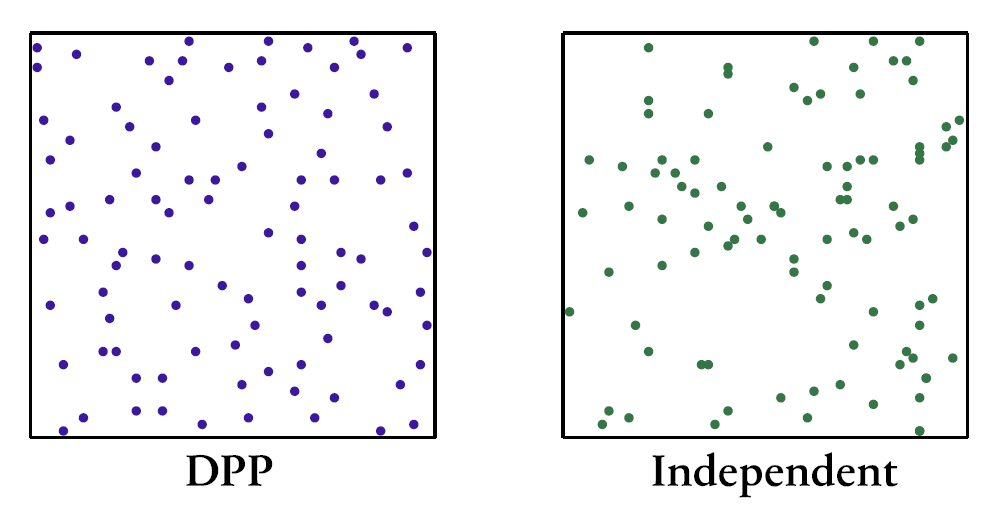
\includegraphics[width=0.6\linewidth]{pics/dpp_vs_iid.png}
    \caption{(left) A set of points in the plane drawn from a DPP, with $K_{i j}$ inversely related to the distance between points $i$ and $j$. (right) The same number of points sampled independently using a Poisson point process , which results in random clumping.}
    \label{fig_dpp_vs_iid}
\end{figure}


\vspace{10cm}
